\chapter{Konzeption und Entwurf von Reforge}
\section{Anforderungsanalyse}
Eine Anforderungsanalyse ist ein essenzieller Schritt im Entwicklungsprozess von Softwareprojekten. Sie stellt sicher, dass alle notwendigen Anforderungen erfasst, dokumentiert und verstanden werden, bevor mit der eigentlichen Entwicklung begonnen wird. Im Rahmen dieses Projekts wird das Modell der Anforderungsanalyse nach Kleuker herangezogen. \cite[S.51 ff.]{kleuker2013anforderungsanalyse}

\subsection{Funktionale Anforderungen}
\label{subs:funktionaleAnfoderungen}
 Funktionale Anforderungen werden üblicherweise durch die Modalverben „muss“, „soll“ und „wird“ klassifiziert, die den Erfüllungsgrad der jeweiligen Anforderung definieren. Anforderungen von wichtiger Bedeutung für das System werden mit „muss“ beschrieben, da deren Erfüllung für den Projekterfolg unverzichtbar ist. Anforderungen, die als hilfreich oder wünschenswert gelten, jedoch nicht zwingend erforderlich sind, werden mit „soll“ gekennzeichnet. Anforderungen, die als potenzielle Erweiterungen für die Zukunft betrachtet werden, werden mit „wird“ formuliert. Im Folgenden werden alle funktionalen Anforderungen des Projekts \textit{Reforge} nach dieser Klassifizierung beschrieben. \cite[S.71 ff.]{kleuker2013anforderungsanalyse}

 Des Weiteren werden, ähnlich zu Raus Vorgehensweise, für die einzelnen Anforderungen Akzeptanzkriterien formuliert, um diese präziser zu definieren. Ein Akzeptanzkriterium ist eine spezifische Bedingung, die erfüllt sein muss, damit eine Anforderung als vollständig umgesetzt gilt. \cite[S.49]{rau2016agile}

\subsubsection{A1 DOCX- und LaTeX-Input}

A1.1 Textextraktion: Das Programm muss in der Lage sein, den Textinhalt aus den hochgeladenen Dokumenten zu extrahieren. Es werden nur Abschlussarbeiten im DOCX-Format oder als LaTeX-ZIP-Ordner entgegengenommen. Die LaTeX-ZIP-Ordner müssen zudem eine Hauptdatei enthalten. Damit wird sichergestellt, dass der Text für die weitere Bearbeitung zur Verfügung steht. Diese Anforderung gilt als erfüllt, wenn der extrahierte Text den gesamten Inhalt des Dokuments umfasst und keine wesentlichen Teile auslässt.
 
\subsubsection{A2 \ac{LLM} Textzusammenfassung}
Die Anforderungen in „\ac{LLM} Textzusammenfassung“ umfasst mehrere Funktionen, die sicherstellen, dass Texte von dem \ac{LLM} verarbeitet und zusammengefasst werden können.

A2.1 Zusammenfassung-Generator: Das Programm muss mithilfe eines \ac{LLM}s in der Lage sein, eine Zusammenfassung der hochgeladenen Inhalte zu generieren. Das Akzeptanzkriterium dieser Anforderung ist erfüllt, wenn die generierten Zusammenfassungen die Hauptaussagen des Originaldokuments widerspiegeln.

A2.2 Textaufteilung zur Vermeidung von Token-Limits: Das Programm muss in der Lage sein, große Textmengen in kleinere Segmente aufzuteilen und diese nach der Verarbeitung wieder zu einem vollständigen Text zusammenzufügen. Diese Anforderung gilt als akzeptiert, wenn der Prozess der Aufteilung und Zusammenführung die inhaltliche Reihenfolge des ursprünglichen Textes nicht verändert. Außerdem muss die Segmentierung für sowohl \ac{DOCX} als auch LaTeX funktionieren.

A2.3 \ac{API}-Schnittstelle für \ac{LLM}: Das Programm muss in der Lage sein, mit der OpenAI-\ac{API} zu kommunizieren. Das Akzeptanzkriterium dieser Anforderung ist erfüllt, wenn die Anwendung eine stabile Verbindung zur OpenAI-\ac{API} aufbauen kann und Anfragen ohne Fehler übermitteln kann.

\subsubsection{A3 \ac{DOCX}- und LaTeX-Output}
Die Anwendung bietet zwei Exportfunktionen für die Ausgabe des generierten Textes. Sie bietet die Konvertierung in ein Word-Dokument und in ein LaTeX-Dokument.

A3.1 \ac{DOCX}-Ausgabe: Die Anwendung muss den generierten Text in das .docx-Format konvertieren können und dabei die Forschungsbericht-Vorlage verwenden. Als Akzeptanzkriterium wird sichergestellt, dass der entstandene Text in Microsoft Word fehlerfrei lesbar und editierbar ist. 

A3.2 LaTeX-Ausgabe: Die Anwendung muss den generierten Text zu .tex konvertieren können und dabei die IEEEtran-Vorlage berücksichtigen. Diese Anforderung gilt als akzeptiert, sobald das entstandene .tex-Dokument fehlerfrei kompilierbar ist.

\subsubsection{A4 Multi-lingual (EN/DE)}
A4.1 Sprachauswahl: Der Benutzer muss auswählen können, in welcher Sprache der Bericht erstellt wird. Diese Auswahl muss unabhängig von der Eingabesprache des Inputs erfolgen. Diese Anforderung gilt als akzeptiert, wenn der Nutzer eine Sprachauswahl tätigen kann.

A4.2 Automatische Übersetzung: Die Anwendung muss eine automatisierte Übersetzungsfunktion für englische und deutsche Versionen des Techreports haben. Sobald die vom Benutzer gewählte Sprache im generierten Endprodukt vorliegt, ist diese Anforderung erfüllt.

\subsubsection{A5 Sonstige funktionale Anforderungen}
A5.1 Benutzeroberfläche: Die Anwendung muss einen Upload-Bereich für die Dokumente haben. Die Anwendung muss Eingabefelder für die Report-Metadaten wie Titel, Autor und Datum haben. Die Anwendung muss eine Auswahl der Ausgabeformate und der gewünschten Sprache haben. Das Akzeptanzkriterium dieser Anforderung ist erfüllt, wenn alle Oberflächenelemente funktionsfähig sind.
    
A5.2 Fortschrittsanzeige: Die Anwendung soll den Fortschritt während der Textverarbeitung und des Exports anzeigen. Diese Anforderung gilt als erfüllt, sobald eine Fortschrittsanzeige zu sehen ist.

A5.3 Export-Funktion: Die Anwendung muss die Möglichkeit bieten, die generierten Berichte herunterzuladen. Das Akzeptanzkriterium dieser Anforderung ist erfüllt, wenn ein Dokument erfolgreich lokal gespeichert werden konnte.

A5.4 Fehlerbehandlung: Die Anwendung sollte auf Fehlersituationen wie ungültige Dateiformate oder \ac{API}-Ausfälle reagieren und dem Benutzer entsprechende Meldungen anzeigen. Diese Anforderung gilt als akzeptiert, wenn der Benutzer in der Lage ist Fehler-Rückmeldungen zu sehen.

\subsection{Nicht-Funktionale Anforderungen}
Die nicht-funktionalen Anforderungen sind entscheidend dafür, dass ein funktionstüchtiges und benutzerfreundliches Software-Projekt entsteht, das den Qualitätsstandards entspricht. \cite[S.77]{kleuker2013anforderungsanalyse}

Zur Klassifikation der nicht-funktionalen Anforderungen wird das FURPS-Modell herangezogen. FURPS steht dabei für Funktionalität, Usability, Reliability, Performance und Supportability. \cite{jamwal2010analysis}

Die Funktionalität umfasst Funktionen des Systems und Sicherheitsvorkehrungen:
\begin{itemize}
    \item Plattformunabhängigkeit: Die Anwendung sollte auf verschiedenen Betriebssystemen und in allen gängigen Webbrowsern konsistent funktionieren.
    \item Responsive Design: Die Benutzeroberfläche sollte sich dynamisch an verschiedene Bildschirmgrößen anpassen und sowohl auf Desktops als auch auf mobilen Geräten gut nutzbar sein.
\end{itemize}

Die Usability fokussiert sich auf die Benutzerfreundlichkeit:
\begin{itemize}
    \item Intuitive Benutzeroberfläche: Die Anwendung sollte einfach und intuitiv zu bedienen sein. Die wichtigsten Funktionen wie zum Beispiel der Upload sollten leicht zugänglich sein.
    \item Fehlermeldungen: Die Anwendung sollte verständliche Fehlermeldungen haben, welche dem Benutzer Hinweise geben, wie Fehler behoben werden können.
\end{itemize}

Die Reliability bezieht sich auf die Zuverlässigkeit des Systems:
\begin{itemize}
    \item Fehlertoleranz: Die Anwendung sollte in der Lage sein, bei einzelnen Fehlern wie zum Beispiel falsche Benutzereingaben weiterzufunktionieren.
    \item \ac{LLM} Verbindungsfehler: Die Anwendung sollte den Benutzer informieren, wenn die Verbindung zur \ac{LLM} im Backend fehlschlägt.
\end{itemize}

Die Performance beschreibt Anforderungen an Geschwindigkeit und Effizienz:
\begin{itemize}
    \item Reaktionszeit: Die Anwendung sollte in der Lage sein, Dokumente schnell zu verarbeiten und Zusammenfassungen in höchstens einer Minute zu generieren.
    \item Effiziente Verarbeitung: Trotz der Arbeit mit großen Textdokumenten sollte die Anwendung so optimiert sein, dass sie effizient mit Ressourcen wie Speicher umgeht.
\end{itemize}

Die Supportability definiert die Wartbarkeit und Erweiterbarkeit des Systems:
\begin{itemize}
    \item Zukünftige Formate: Die Architektur der Anwendung sollte so gestaltet sein, dass leicht neue Exportformate oder Vorlagen hinzugefügt werden können, ohne große Änderungen am bestehenden System vorzunehmen.
    \item \ac{API}-Erweiterbarkeit: Die Integration neuer \ac{API}s, zum Beispiel für Übersetzungen oder andere \ac{LLM}-\ac{API}s, sollte leicht möglich sein.
\end{itemize}
\section{Wireframes}
\label{sec:wireframe}
Ein wichtiges Mittel des Prototypings ist die Erstellung eines Wireframes. Ein Wireframe ist eine vereinfachte grafische Darstellung der Benutzeroberfläche einer Anwendung. Wireframes werden verwendet, um die grundlegende Struktur und Funktionalität einer Website oder Anwendung vor dem eigentlichen Design und der Implementierung zu visualisieren. Sie zeigen, wie Informationen angeordnet sind, welche Elemente auf der Benutzeroberfläche vorhanden sind und wie die Navigation im System funktioniert. Wireframes helfen, Ideen zu kommunizieren, Feedback von Nutzern oder Stakeholdern einzuholen und sicherzustellen, dass das Layout der Benutzeroberfläche den Anforderungen entspricht. \cite[S.119]{preim2015interaktive}

Die Abbildung \ref{fig:wireframe_upload} zeigt den Entwurf der Upload-Seite, in der alle wesentlichen Elemente skizziert sind. Zentrales Element der Seite ist der File-Upload-Button, über den die Benutzer ihre Dokumente hochladen können. Direkt darunter befinden sich die Eingabefelder für Autor und Titel, mit denen das generierte Dokument beschriftet wird. Es folgen Radiobuttons zur Auswahl des Ausgabeformats, wobei der Nutzer zwischen LaTeX und \ac{DOCX} wählen kann. Daneben ist eine Sprachauswahl eingebettet, die ebenfalls über Radiobuttons gesteuert wird und zwischen Deutsch und Englisch unterscheidet. Schließlich gibt es noch einen Start-Button, mit dem der Benutzer die Generierung des Berichts startet. Die Elemente wurden so angeordnet, dass die Seite wie ein Formular aussieht, das von oben nach unten ausgefüllt werden muss. 

\begin{figure}[H]
\centering
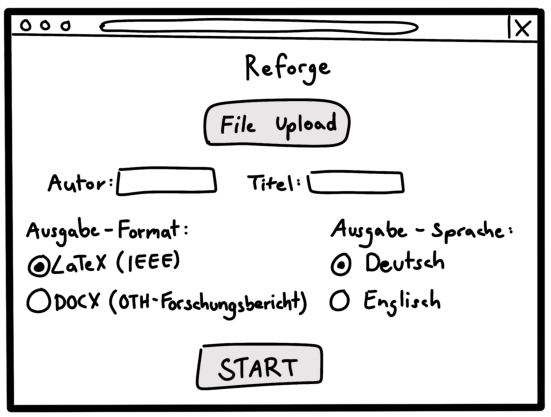
\includegraphics[width=0.5\linewidth]{Images/wireframe_upload.pdf}\\
\caption{Wireframe für die Upload-Seite von Reforge}
\label{fig:wireframe_upload}
\end{figure}

Die Abbildung \ref{fig:wireframe_download} zeigt die Hauptfunktionen der Download-Seite, die sich in zwei Buttons zusammenfassen lassen. Der eine Button ist für das Herunterladen der generierten Datei zuständig. Mit dem anderen Button kehrt der Benutzer zur Upload-Seite zurück, falls er sich entscheidet, einen weiteren Bericht zu generieren. Diese beiden Wireframes bilden eine gute Grundlage für die Entwicklung und stellen sicher, dass die Anordnung der Elemente optimal geplant wird.

\begin{figure}[H]
\centering
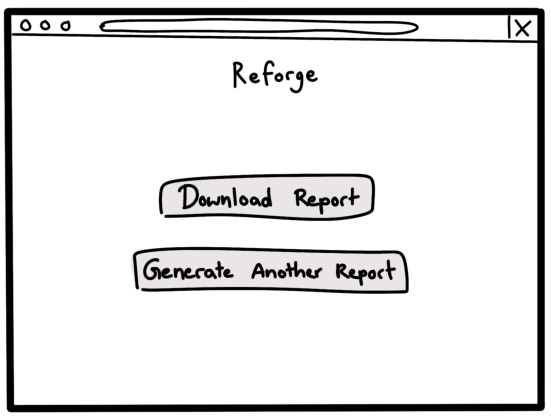
\includegraphics[width=0.5\linewidth]{Images/wireframe_download.pdf}\\
\caption{Wireframe für die Download-Seite von Reforge}
\label{fig:wireframe_download}
\end{figure}

\section{Auswahl des LLMs für die Textzusammenfassung}
\label{4.3_LLM}
Die Auswahl eines geeigneten \ac{LLM}s für die Textzusammenfassung ist ein wesentlicher Schritt, um die Qualität der erzeugten Berichte zu gewährleisten. Für dieses Projekt wurde das von OpenAI entwickelte \ac{GPT}-3.5-turbo ausgewählt, da dieses \ac{LLM} entscheidende Vorteile gegenüber anderen \ac{LLM}s bietet.

Ein großer Vorteil ist, dass die \ac{LLM}s von OpenAI nicht selbst gehostet werden müssen. Dies erleichtert die Integration der \ac{LLM}s in das System. Zudem verfügt OpenAI über eine gut dokumentierte \ac{API}, die sich leicht in die bestehende Systemarchitektur integrieren lässt, was die Entwicklungszeit verkürzt. Darüber hinaus zeichnen sich die von OpenAI entwickelten Modelle durch Präzision und ein tiefes Verständnis komplexer Textstrukturen aus. Sie ermöglichen die Erstellung von kontextbezogenen Zusammenfassungen, was insbesondere bei der Verarbeitung wissenschaftlicher Texte eine große Rolle spielt. 

OpenAI beschreibt in der Dokumentation, wie ein REST-\ac{API}-Aufruf gestaltet werden kann. Dieses Beispiel aus der offiziellen OpenAI Dokumentation ist in Listing \ref{lst:OpenAI_API_Example} dargestellt. Hier ist zu sehen, dass im \ac{API}-Request ein Modell definiert werden muss. OpenAI bietet viele verschiedene \ac{LLM}s an, die alle unterschiedliche Stärken und Schwächen besitzen. Eine Übersicht aller aktuell von OpenAI angebotenen Modelle ist auf der offiziellen Webseite\footnote[1]{OpenAI Modell Übersicht: \href{https://platform.openai.com/docs/models}{https://platform.openai.com/docs/models}} zu finden. Darunter ist das \ac{GPT}-4o-mini Model zu finden, welches hier in diesem Beispiel von OpenAI verwendet wird. Dieses Modell zeichnet sich damit aus günstig und schnell für kleinere Aufgaben zu sein. 

\begin{listing}[H]
\begin{minted}[
frame=lines,
bgcolor=base,
fontsize=\footnotesize,
linenos
]
{javascript}
import OpenAI from "openai";
const openai = new OpenAI();

const completion = await openai.chat.completions.create({
    model: "gpt-4o-mini",
    messages: [
        { role: "system", content: "You are a helpful assistant." },
        {
            role: "user",
            content: "Write a haiku about recursion in programming.",
        },
    ],
});

console.log(completion.choices[0].message);
\end{minted}
\caption{OpenAI REST-\ac{API}-Example \cite{openai_quickstart}}
\label{lst:OpenAI_API_Example}
\end{listing}

Als nächstes muss eine Nachricht, der sogenannte Prompt, definiert werden, welche das \ac{LLM} bei der Bearbeitung der Anfragen unterstützt. Diese Nachricht ist in mehrere Rollen unterteilt. Es gibt die \texttt{system}-Rolle, die dem \ac{LLM} Anweisungen gibt, was es erledigen und wie es reagieren soll. Die \texttt{user}-Rolle beschreibt, was der Output sein soll. Diese Rolle ist vergleichbar mit dem Benutzer im Chat\ac{GPT}, der im Chat eingibt, was er als Ergebnis haben möchte. \cite{openai_quickstart}

Im Vergleich dazu sind andere Modelle, wie die von Hugging Face angebotenen \ac{LLM}s, zwar ebenfalls leistungsfähig, erfordern aber oft eine umfangreiche Feinabstimmung und eine eigene Hosting-Infrastruktur, was den Aufwand für das Projekt erhöht hätte. Die Entscheidung für OpenAI basierte daher auf einer Abwägung zwischen einfacher Integration, hoher Sprachqualität und möglichst effizienter Entwicklungszeit.


\section{Systemarchitektur}

In diesem Abschnitt wird zunächst die Architektur des Systems erläutert. Anschließend wird auf die Speicherung der Daten eingegangen. Schließlich wird ein Sequenzdiagramm vorgestellt, welches den Upload Ablauf visualisiert.

\begin{figure}[H]
\centering
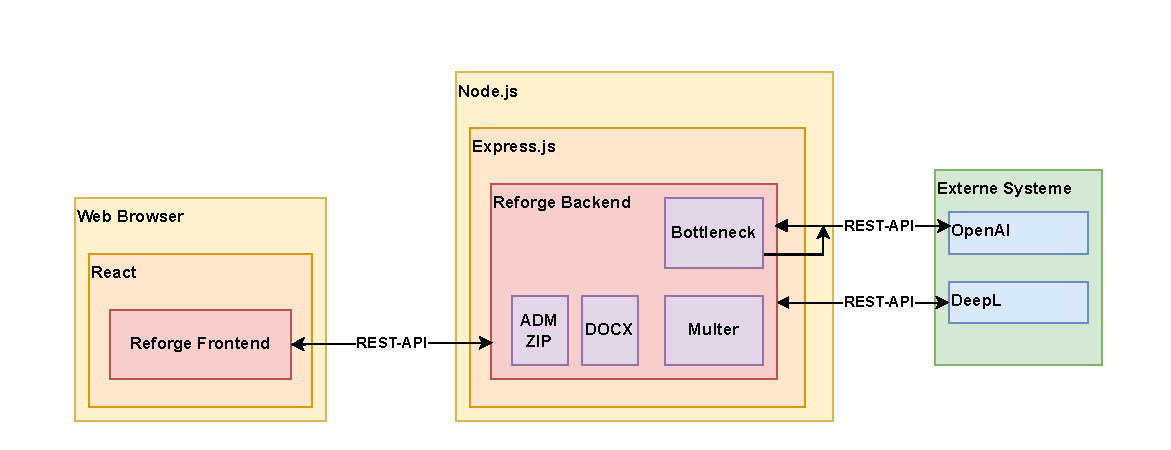
\includegraphics[width=1\linewidth]{Images/Systemarchitektur.pdf}\\
\caption{Systemarchitektur von Reforge}
\label{fig:sys_architektur}
\end{figure}

Die Abbildung \ref{fig:sys_architektur} zeigt den Entwurf für die Systemarchitektur der Anwendung Reforge. Diese Architektur setzt auf eine RESTful \ac{API}, die eine Kommunikation zwischen Frontend, Backend und den externen Systemen ermöglicht. Dabei werden Daten über \ac{HTTP}-Methoden wie \textbf{POST} ausgetauscht.

Das Frontend basiert auf React und läuft im Webbrowser des Benutzers. Es stellt die Benutzerschnittstelle bereit, über die alle Interaktionen erfolgen. Die Benutzereingaben werden über die RESTful \ac{API} an das Backend übertragen. 

Das Backend, ausgeführt mit Node.js und Express.js, übernimmt die serverseitige Logik und verarbeitet die Anfragen, die vom Frontend gesendet werden. Die Verwaltung der Dateispeicherung erfolgt mithilfe von Middleware wie Multer \footnote[1]{Multer: \href{https://expressjs.com/en/resources/middleware/multer.html}{https://expressjs.com/en/resources/middleware/multer.html}}, das die Daten temporär im Arbeitsspeicher zwischenspeichert, bevor sie weiterverarbeitet werden. Für das Management und die Verarbeitung von Dateien verwendet das Backend ADM-ZIP\footnote[2]{ADM-ZIP: \href{https://www.npmjs.com/package/adm-zip}{https://www.npmjs.com/package/adm-zip}} für das Handling von ZIP-Dateien sowie DOCX\footnote[3]{DOCX: \href{https://www.npmjs.com/package/docx}{https://www.npmjs.com/package/docx}} zur Formatierung und Erstellung von Word-Dokumenten. Diese Tools ermöglichen es dem Backend, die hochgeladenen Inhalte im gewünschten Format bereitzustellen.

Zur Erweiterung der Funktionalität greift die Anwendung auf externe Systeme zurück. Die OpenAI \ac{API}\footnote[4]{OpenAI API: \href{https://platform.openai.com/docs/overview}{https://platform.openai.com/docs/overview}} wird für die Verarbeitung und Generierung von Textinhalten genutzt, während die DeepL \ac{API}\footnote[5]{DeepL API: \href{https://www.deepl.com/de/pro-api/}{https://www.deepl.com/de/pro-api/}} die Übersetzung von Überschriften innerhalb der Anwendung übernimmt. Da OpenAI bei zu vielen Anfragen in kurzer Zeit blockiert, wird Bottleneck\footnote[6]{Bottleneck: \href{https://www.npmjs.com/package/bottleneck}{https://www.npmjs.com/package/bottleneck}} eingesetzt, um die Anfragerate für die OpenAI \ac{API} gezielt zu drosseln.

\subsection{Speicherung von Daten}
Im Rahmen dieses Projekts wurde bewusst darauf verzichtet, eine Datenbank zu implementieren, da dies nicht Teil der Anforderungen war und den Projektrahmen gesprengt hätte. Stattdessen erfolgt die Speicherung der Daten aktuell nur in Form einer temporären Zwischenspeicherung innerhalb der Anwendung.

Für die Zwischenspeicherung kommt die Middleware Technologie Multer zum Einsatz, die es ermöglicht, hochgeladene Dateien für die Dauer der Verarbeitung zu speichern und anschließend weiterzuleiten. Hierfür wird die \textbf{memoryStorage}-Funktion von Multer verwendet, welche die Dateien als Buffer speichert. Bei dieser Methode enthält das Dateifeld ein Buffer-Objekt, welches die gesamte Datei im Arbeitsspeicher hält. Diese Vorgehensweise ist effizient für kleinere Dateien. Der Arbeitsspeicher kann jedoch bei großen oder sehr vielen kleinen Dateien überlastet werden, weshalb die Speicherlast im Auge behalten werden sollte. \cite{multer}

\subsection{Verlauf des Uploads in Reforge}

Um die zeitliche Abfolge von Interaktionen zwischen den Komponenten eines Systems darzustellen, eignet sich das Sequenzdiagramm. Es gehört zu den Verhaltensdiagrammen der \ac{UML} und ist eines der vier Interaktionsdiagramme. Sequenzdiagramme zeigen, wie die Kommunikation zwischen verschiedenen Systemkomponenten abläuft, indem sie die gesendeten Nachrichten und deren zeitliche Reihenfolge veranschaulichen \cite{rumpe2004sequenzdiagramme}. Mit Hilfe von einem Sequenzdiagrammen soll nun der Prozess des Uploadens von Dateien erklärt werden.

Abbildung \ref{fig:Sequenzdiagramm} zeigt das Sequenzdiagramm des Upload-Prozesses in der Anwendung. Der Ablauf beginnt im Frontend, wo der Benutzer eine Datei hochlädt. Das Backend empfängt die Datei, liest sie und bereitet den Text für die weitere Verarbeitung vor. Anschließend wird der vorbereitete Text an die OpenAI \ac{API} gesendet, um eine Zusammenfassung zu generieren. Sobald die Zusammenfassung erstellt wurde, kehrt diese zum Backend zurück. Danach wird der Text an die Deepl \ac{API} gesendet, um die Überschriften zu übersetzen. Die übersetzten und verarbeiteten Daten werden schließlich an das Frontend zurückgesendet, sodass die fertige Datei dem Benutzer zur Verfügung gestellt werden kann.

\begin{figure}[H]
\centering
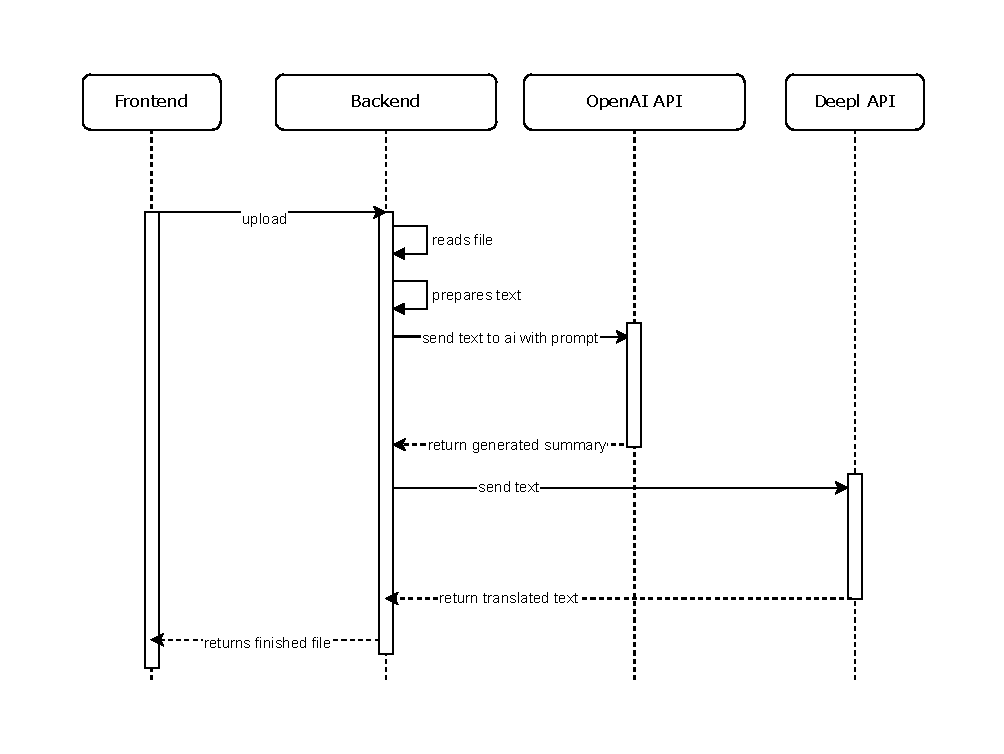
\includegraphics[width=1\linewidth]{Images/Sequenzdiagramm.pdf}\\
\caption{Sequenzdiagramm des Upload-Prozesses}
\label{fig:Sequenzdiagramm}
\end{figure}


